\documentclass{standalone}
\usepackage{tikz}
\usepackage{pgfplots}
\pgfplotsset{width=32cm,height=18cm,compat=1.3}
\pgfplotsset{every tick label/.append style={font=\Huge}}
\usepackage{filecontents}
\usepgfplotslibrary{fillbetween}

\usetikzlibrary{patterns}

\definecolor{citrine}{rgb}{0.89, 0.82, 0.04}

\begin{document}
	\centering
		\vspace{1.5em}
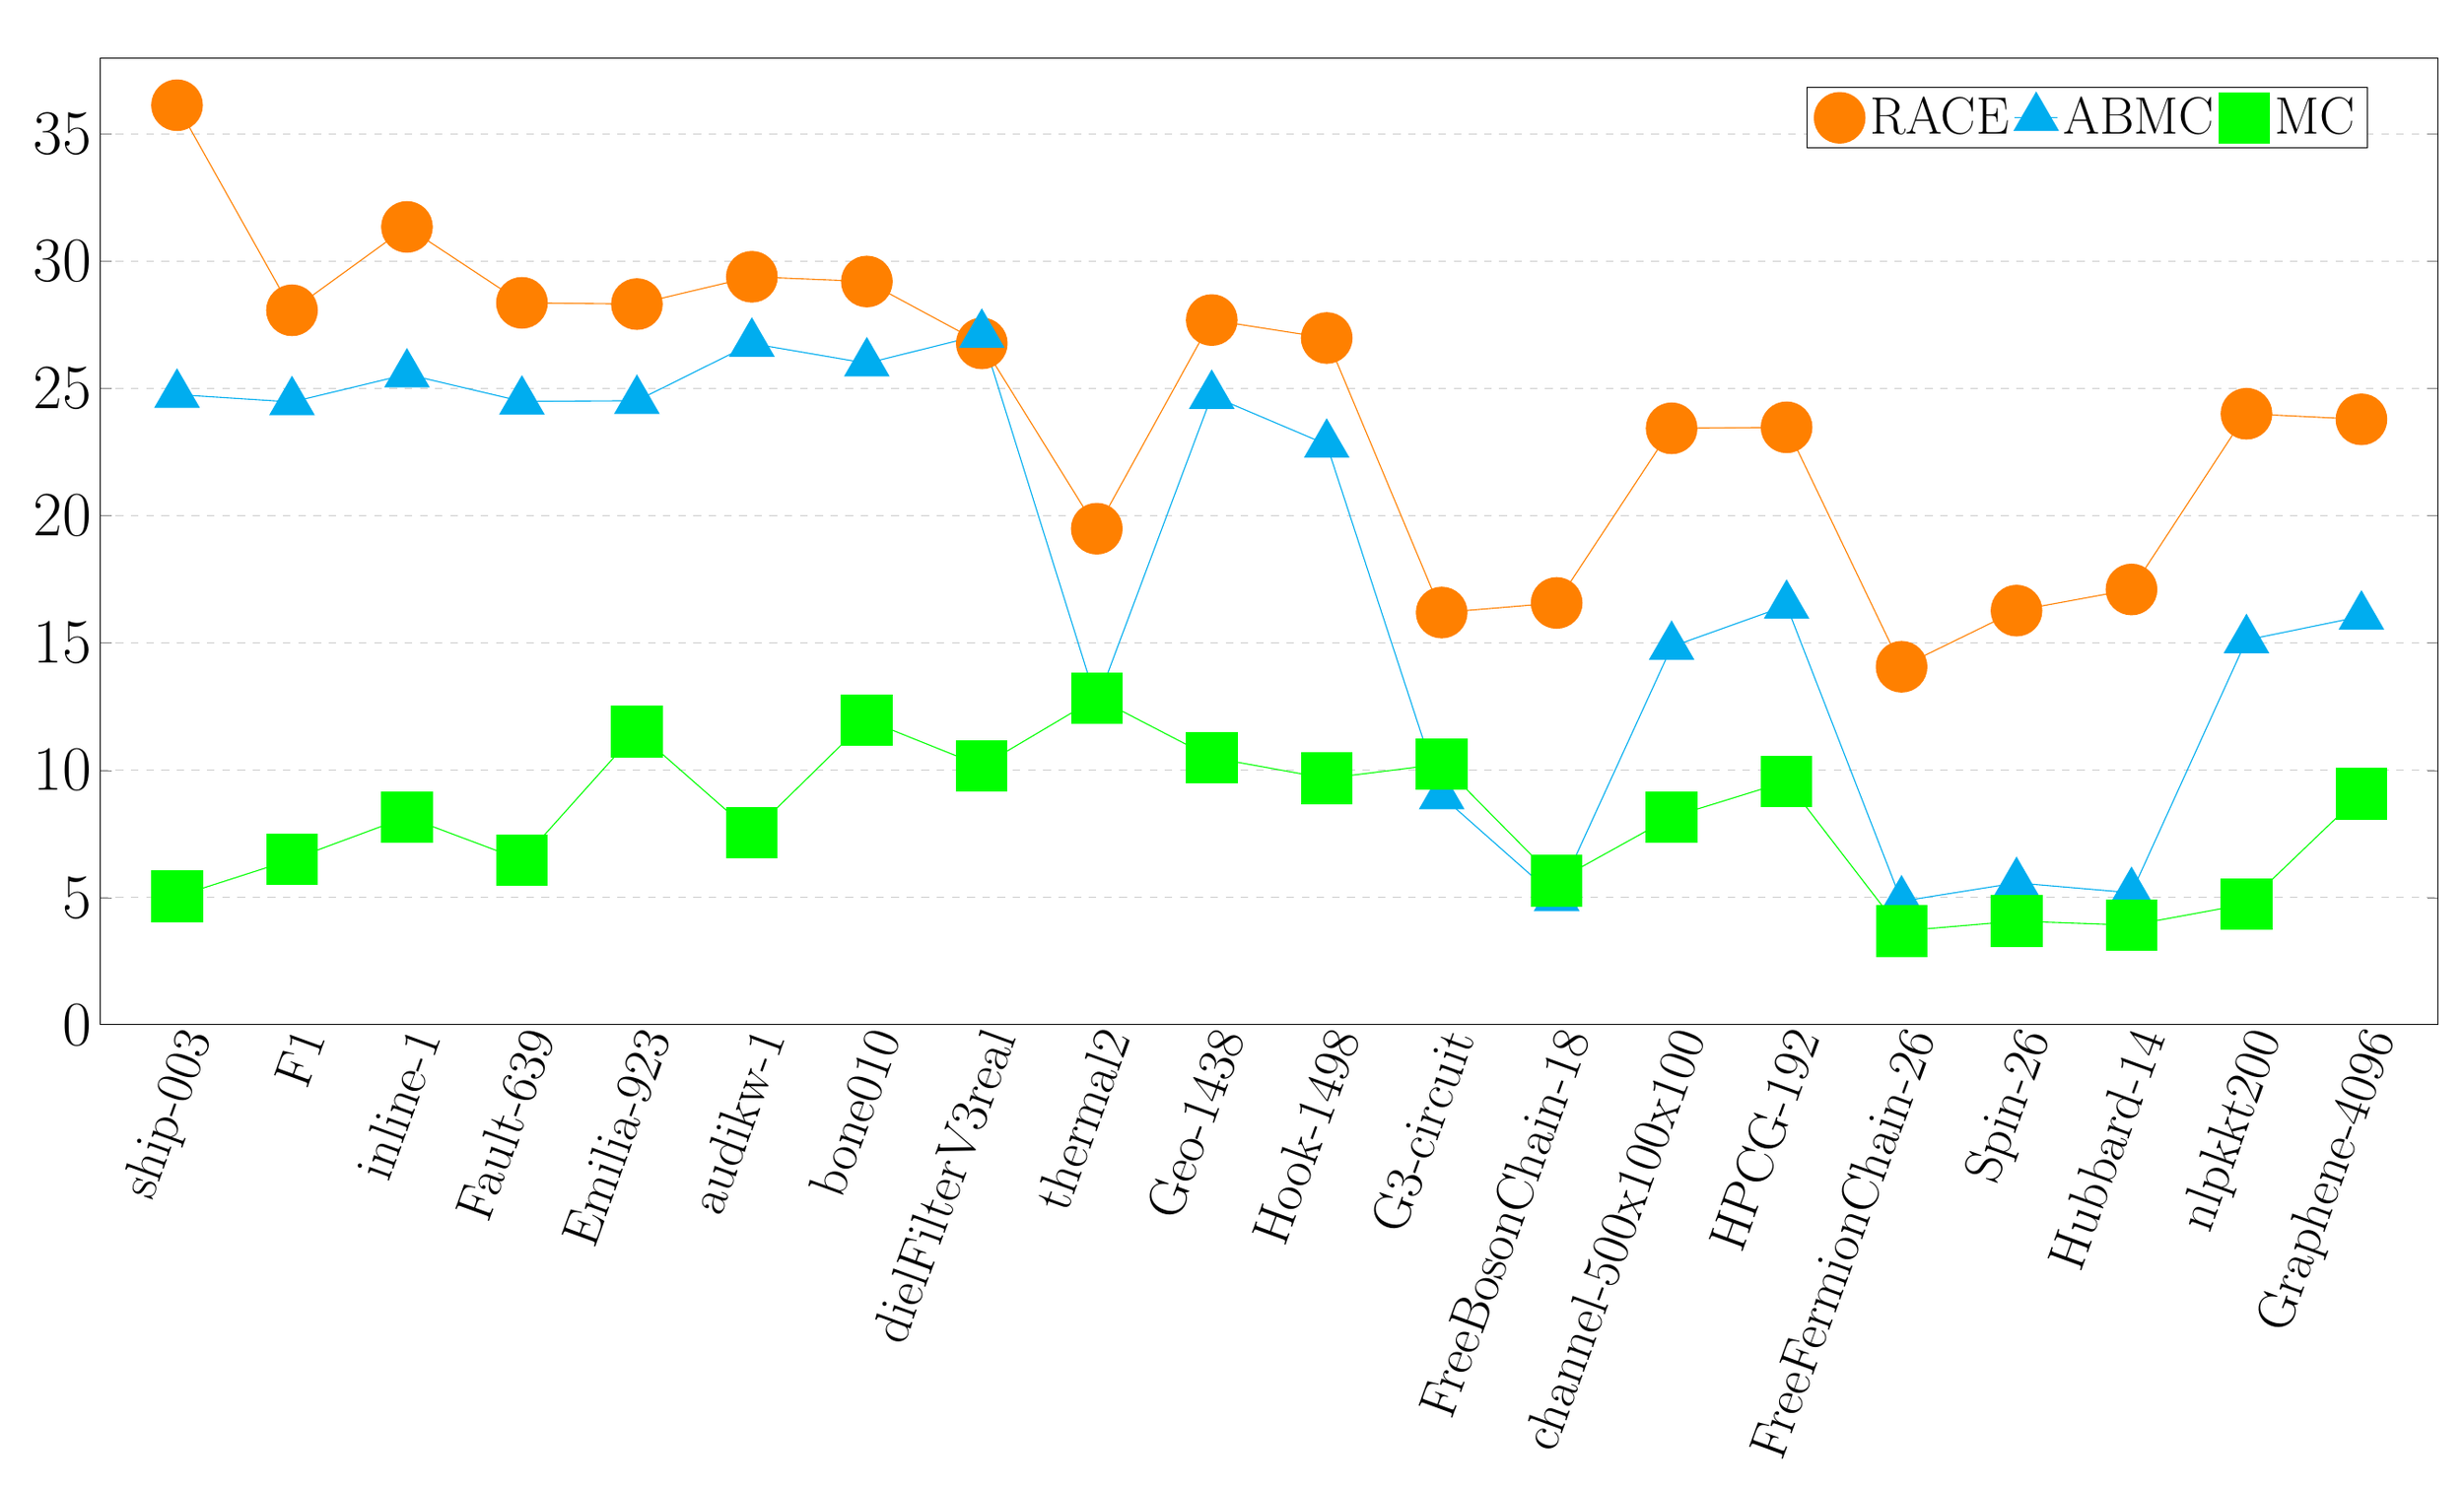
\begin{tikzpicture}
		%	\node at (13.25,15) {\LARGE{}};
			\begin{axis}[
		%	xmin=0.25, xmax=7.25,
		ymin=0, %ymax=3.25,
		ymax=38,
		xtick={1, 2, 3, 4, 5, 6, 7, 8, 9, 10, 11, 12, 13, 14, 15, 16, 17, 18, 19, 20, 21, 22, 23, 24, 25, 26, 27, 28, 29, 30, 31},
		%	ytick={0,0.5,1,1.5,2,2.5,3},
		xticklabels={ ship-003, F1, inline-1, Fault-639, Emilia-923, audikw-1, bone010, dielFilterV3real, thermal2, Geo-1438, Hook-1498, G3-circuit, FreeBosonChain-18, channel-500x100x100, HPCG-192, FreeFermionChain-26, Spin-26, Hubbard-14, nlpkkt200, Graphene-4096},
		width  = 34cm,
		height = 15cm,
		major x tick style = transparent,
		%	minor ytick={1, 5, 10, 15, 20, 25, 30 ,35,40},
		grid = minor,	
		%add_bar_commands
		ymajorgrids = true,
		grid style={dashed, gray!40},
		%ylabel = {\Huge{Perf (GF/s)}},
		%	symbolic x coords={Graphene-2048-2048, Graphene-4096-4096, Spin-24-24-24},
		x tick label style={rotate=70, anchor=north east, inner sep=0mm, font={\huge}},
		%	tick label style={font={\Huge}},
		scaled y ticks = false,
		enlarge x limits=0.035,
		legend cell align=left,
		legend style={font=\huge},
		legend columns=-1,
		legend style={
			%at={(1,1.05)},
			%anchor=south east,
			%column sep=1ex,
			legend pos=north east
		},
		%spl_legend_code
		title= {\Huge\scalebox{1.5}{{}}}
		]

\addplot[name path=RACE-SymmSpMV, mark=*, mark size=10pt, mark options={orange}, draw=orange ] plot coordinates{(1,36.140175) (2,28.080251) (3,31.356939) (4,28.372987) (5,28.323231) (6,29.396679) (7,29.210280) (8,26.778583) (9,19.496395) (10,27.696097) (11,26.990050) (12,16.199662) (13,16.577436) (14,23.441453) (15,23.480804) (16,14.069287) (17,16.275497) (18,17.107030) (19,24.014713) (20,23.793009)};
\addplot[ mark=triangle*, mark size=10pt, mark options={cyan}, draw=cyan ] plot coordinates{ (1,24.768035) (2,24.475683) (3,25.563859) (4,24.498829) (5,24.526497) (6,26.773144) (7,25.998597) (8,27.122656) (9,12.667727) (10,24.722981) (11,22.803733) (12,8.987108) (13,4.988385) (14,14.858202) (15,16.473370) (16,4.853501) (17,5.575532) (18,5.185500) (19,15.120960) (20,16.047102)};
\addplot[ mark=square*, mark size=10pt, mark options={green}, draw=green ] plot coordinates{ (1,5.041221)  (2,6.494727) (3,8.166534) (4,6.471868) (5,11.516064) (6,7.549159) (7,11.979405) (8,10.165285) (9,12.841705) (10,10.498566) (11,9.682819) (12,10.243942) (13,5.660339)  (14,8.163804) (15,9.562151) (16,3.686573) (17,4.074622) (18,3.911298) (19,4.742299) (20,9.073864)};
	%addplot cmd

	\legend{RACE, ABMC, MC}

	\end{axis}			
\end{tikzpicture}

\end{document}

